\documentclass[12pt]{article} % Document class, and 12 pt

% Packages
\usepackage[utf8]{inputenc} % Input encoding
\usepackage[T1]{fontenc}    % Output encoding
\usepackage{textcomp} % print euro symbol
\usepackage{booktabs}
\usepackage{enumitem}
\usepackage{amssymb}
\usepackage{xcolor}
\usepackage{listings}
\usepackage{graphicx} % insert picture
\usepackage{array}
\usepackage{setspace}
\usepackage{titlesec} % make section 12pt and bold
\usepackage{natbib} % Harvard reference format
\usepackage[hang, bottom]{footmisc} % no space in footnote
\usepackage{hyperref}
\usepackage{tikz} % draw a text structure

% make sections pt 12 and bold
\titleformat{\section}{\bfseries\fontsize{12}{14}\selectfont\centering}{\thesection}{1em}{}
% no space between sections
\titlespacing{\section}{0pt}{\parskip}{-\parskip}
% make subsections pt 12 and bold
\titleformat{\subsection}{\bfseries\fontsize{12}{14}\selectfont}{\thesection}{1em}{}
% no space btween subsections
\titlespacing{\subsection}{0pt}{\parskip}{-\parskip}

\doublespacing
\setlength{\parskip}{\baselineskip}

\definecolor{github-light-bg}{RGB}{255, 255, 255}
\definecolor{github-light-fg}{RGB}{3, 102, 214}
\definecolor{github-light-yellow}{RGB}{128, 102, 0}
\definecolor{github-light-orange}{RGB}{170, 0, 17}
\definecolor{github-light-purple}{RGB}{102, 51, 153}
\definecolor{github-light-cyan}{RGB}{0, 128, 128}
\definecolor{github-light-green}{RGB}{0, 128, 0}
\definecolor{github-light-red}{RGB}{204, 0, 0}

\lstdefinestyle{githublight}{
	backgroundcolor=\color{github-light-bg},
	basicstyle=\color{github-light-fg}\ttfamily,
	commentstyle=\color{github-light-green},
	keywordstyle=\color{github-light-purple},
	numberstyle=\tiny\color{github-light-fg},
	stringstyle=\color{github-light-cyan},
	identifierstyle=\color{github-light-orange},
	emphstyle=\color{github-light-red},
	emph={[2]TRUE,FALSE},
	emphstyle={[2]\color{github-light-yellow}},
	breaklines=true,
	breakatwhitespace=true,
	numbers=left,
	numbersep=5pt,
	stepnumber=1,
	showstringspaces=false,
	frame=single,
	rulecolor=\color{github-light-fg},
	framerule=0.5pt,
	tabsize=4,
	columns=flexible,
	extendedchars=true,
	inputencoding=utf8,
	upquote=true,
}

\lstset{style=githublight}

% Page layout settings
\usepackage[a4paper, margin=2.5cm]{geometry} % Set paper size and margins

\title{Experimental Methods for Social Scientist }
\date{Due: February 18, 2024}
\author{Chenxi Li}

\begin{document}

\begin{figure}[h]
	\centering
	\vspace{-2.5cm}
	\hspace{-8cm}
	
\includegraphics[width=12cm]{Trinity_icon.jpg}  
\end{figure}

\vspace{.5cm}
\begin{center}
    {\fontsize{17.28}{22}\selectfont\bfseries School of Social Sciences and Philosophy} \\
    {\fontsize{17.28}{22}\selectfont\bfseries Assignment Submission Form}
\end{center}

\vspace{.7cm}


\begin{center}
		\begin{tabular}{|>{\arraybackslash}p{4cm}|>{\arraybackslash}p{8cm}|}
			\hline
			Student Name: & Chenxi Li\\
			\hline
			Student ID Number: & 23330541 \\
			\hline
			Programme Title: & Applied Social Data Science \\
			\hline
			Module Title: & Experimental Methods for Social Scientist \\
			\hline
			Assessment Title: & \textit{Experimental design, part 3 }\\
			\hline
			Lecture (s): & Dr Gizem Arikan \\
			\hline
			Date Submitted: & \today \\
			\hline
		\end{tabular}
\end{center}

\vspace{.7cm}

\noindent I have read and I understand the plagiarism provisions in the General Regulations of the University Calendar for the current year, found at:  \url{http://www.tcd.ie/calendar} 
\par
\noindent I have also completed the Online Tutorial on avoiding plagiarism ‘Ready, Steady, Write’, located at \url{http://tcd-ie.libguides.com/plagiarism/ready-steady-write} 

\vspace{.7cm}


\begin{flushleft}
	\begin{minipage}{0.5\linewidth}
		\textbf{Signature:}
		\raisebox{-0.3\height}{
\includegraphics[width=0.6\linewidth]{signature.png}}
	\end{minipage}
\end{flushleft}

\vspace{.3cm}

\noindent \textbf{Date: } \today

\newpage
\begin{center}
	\textbf{POP 77034 Experimental Methods for Social Scientist}\\
	\textbf{Hilary Term 2024}\\
	\textbf{\textit{Experimental design, part 3 (2500 \textendash\ 3000 words)}} \\
	\vspace{.3cm}
	\textbf{Chenxi Li, 23330541}
\end{center}

\vspace{.5cm}

\noindent \textbf{Does Gamification Strategy Improve Social Science Student's Efficiency?}

\vspace{.5cm}

\section*{Abstract}

\vspace{.5cm}

\noindent Gamification, valued at USD 10.2 billion in 2021 and is predicted to reach USD 87.0 billion by 2030
\footnote[1]{
	Global Gamification Market Size, Analyzing Growth and Forecasting Outlook From 2023 \textendash\ 2030, 
	\url{https://www.linkedin.com/pulse/global-gamification-market-size-analyzing-growth/},
	Last accessed: 24 February, 2024
}, 
has led a wave that spans industry, commerce, education, etc. However, most of the research focuses either on non-education areas \citep{caponetto2014gamification}, or only in universities' science projects \citep{stott2013analysis, rabah2018gamification, putz2020can}. This research is bases on the hypothesis that gamification facilitates the students' learning efficiency in humanities and social sciences disciplines within the universities. This study has 126 students in the control group and 126 students in the experimental group, and the effect size is 0.25. Gamification was regarded as an independent variable in the experimental group, while the control group adopted a traditional teaching method.
\newpage

\section*{Introduction}

\vspace{.5cm}

\noindent Since George Hebert Mead presented a series of theories about play, games and generalised other in his class at 1934 \citep{Mead34}, people have begun to search a broad theories of game that look outside the traditional context. With gameing theories progressed and technology development, people started to use game elements into non-game scenarios, which is where the most widely circulated definition of gamification is found \citep{deterding2011game, richards2014beyond, marczewski2013gamification}.
\par
\noindent Gamification technology was already used on a variety range of soocieties including management \citep{deterding2019gamification}, marketing \citep{huotari2012defining}, industrial design \citep{reis2020prospects}, arts curation and treatment \citep{dias2018gamification, pramana2018using}, etc. For education field, however, although there is also a certain amount of gamification research, it is till not as numerous as in the context of a business, which is directly related to profit. Further, most of the research in education is focused on science in universities like physics \citep{rose2016gamification}, engineering \citep{barata2013engaging}, computer science \citep{ibanez2014gamification}, or medical \citep{nevin2014gamification}. There are very few gamification experiments involving the humanities and social science.
\par
\noindent Thus our research idea became clear. This experimental use gamification method as the independent variable and learning outcomes as the dependent variable, and is trying to answer this question: Does gamification strategy improve humanities student's efficiency?
\par
\noindent More specifically, we decided to choose a social science course at Trinity College Dublin, then select a moduele within that course \textit{(Literature Review Part Explans Why)}; operationalise and measure with a series of gamification practice theories under a social sicence context \textit{(See Theoretical Argument Part)}; then randomly divide students into an experimental group and a control group to measure the effects of gamification effects \textit{(See Explanation \& Justification Part)}.

\newpage

\section*{Literature Review}

\vspace{.5cm}

\noindent Broadly speaking, the specific application areas of gamification include two parts, industry and education. The debate in industry section involes to a series of marketing or management strategies, usually is profit and business discussions \citep{huotari2017definition, noorbehbahani2019systematic}, fighting with a philosophy view about humanity, capital and alienation \citep{woodcock2018gamification}. While the education section refers to the experimental in teaching practice, Researchers focused on a range of topics such as which gamification method to use, in which group of students \citep{kocakoyun2018review}, and ultimately how well the gamification works \citep{toda2017dark, alsawaier2018effect}. It is difficult to observe a significant quantitative differences between these two sections. According to Caponetto, \citep{caponetto2014gamification} in research papers, the proportion of educaion and non-education issues is about 52\% 
\footnote[2]{
	Calculated as primary school (3\%) \texttt{+} lower secondary school (4\%) \texttt{+} upper secondary school (2\%) \texttt{+} university (43\%) \texttt{=} education research proportion (52\%).
}
and 48\%, and university students accounted for 43\% of education experiments (Details can be found in Figure1).
\footnote[3]{
	Data source from Caponetto's 2014 study, visualisation recreated by Chenxi.
}.
\begin{figure}[h]
	\centering
	\caption{Literatures in Gamification Subjects Description}
	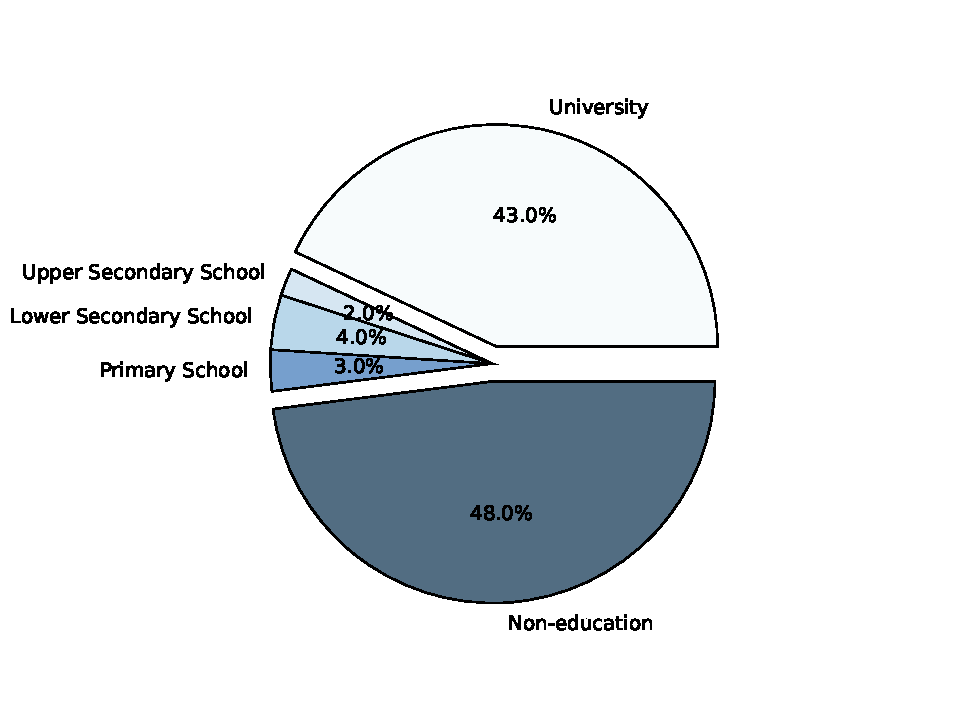
\includegraphics[width=.7\textwidth]
	{literature_statistics.pdf}  
\end{figure}
\newpage
\noindent For those paper focus in education field, a widely held conclusion is that gamification improves students' learning efficiency. In literature reviewing researchs, scholars concluded:
\par
\noindent \textit{The outcomes examined in the studies are mainly focused on quantifiable performance metrics; and the results [\dots] are strongly positively oriented.
} 
\citep{majuri2018gamification}
\\
\noindent \textit{A significant difference was found between the two groups that indicated higher achievement in the experimental group [\dots] Interviews indicated that the students had positive views about gamification strategies.
}
\citep{turan2016gamification}
\par
\noindent A few, but still some scholars argue an opposing view. Toda discuss a negatice effect with leaderboards system in gamification and study enthusiasm\citep{toda2017dark}, and a meta-analysis of gamification also showed that gamification may only work in a short-time term instead of a long-term experimental \citep{kim2021effects}. According a 15 weeks experiment, Van Roy and Zaman also pointed out students will lose their motivatation at the begining of gamification strategy \citep{van2018need}. In 2018, Majuri retrieved the results of past experiments
\footnote[4]{
	Data source from Majuri's 2018 study, visualisation recreated by Chenxi.
}.
(Details can be found in Figure 2), which can provide a view of the distribution of students' reaction \citep{majuri2018gamification}.
\begin{figure}[h]
	\centering
	\caption{Literatures in Gamification Results Description}
	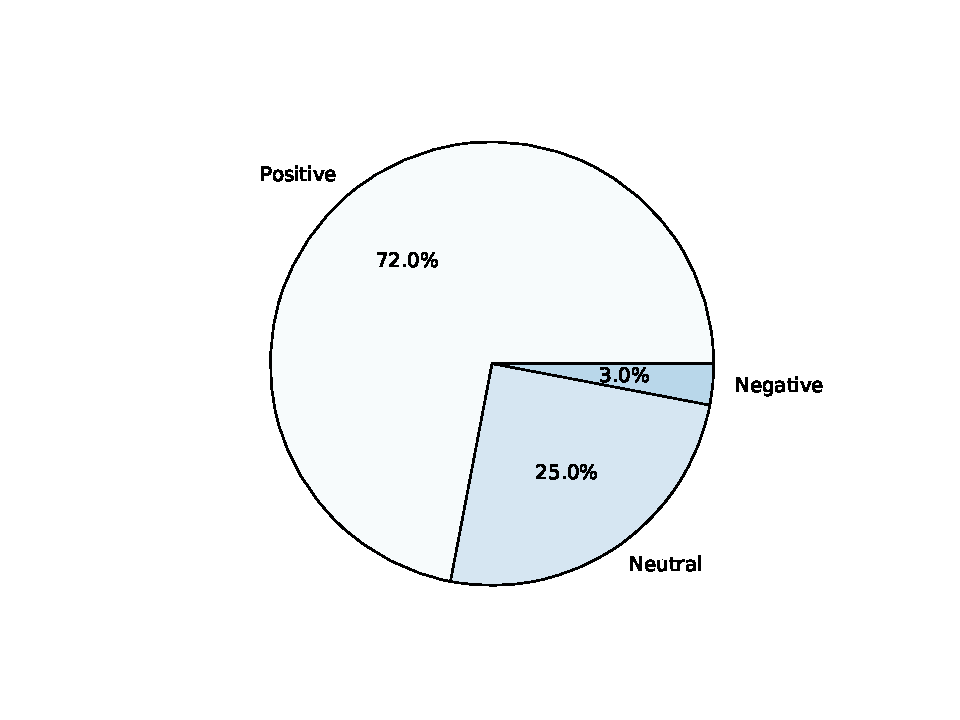
\includegraphics[width=.7\textwidth]
	{results_statistics.pdf}  
\end{figure}
\par 
\noindent Indeed, the subjects of the gamification research \textendash\ that is, the disciplines in which the experiments were carried out \textendash\ were not homogeneous, with science and technology being invested in more by researchers. Most of the evidence scholars have found is in science subjects \citep{kalogiannakis2021gamification}, and some of them are under a science laboratory enviorment \citep{fleischman2016gamification, drace2013gamification}, which will cause a STEM courses limitation \citep{rabah2018gamification} and some potential Hawthorne effects due to the observer being in the lab. In such a scenario, experiments in the liberal arts or social sciences become even more necessary.
\par
\noindent Current gamification experiments in social science field fall in several subjects like gender studies \citep{ortega2019gamification} and historical studies \citep{cozar2016game}. It is also worth mentioning that there are also studies in this field transfer their vision from students to teachers, using gamification to training them for social science teaching content \citep{yildiz2021effect}.  In summary, almost half of the studies focus on industry and the other half on education, and their studies basically show that gamification, especially in scientific disciplines, has a positive impact on students, however, there still exists a dearth of gamification experiments in social science scenarios.

\newpage

\section*{Theoretical Argument}

\vspace{.5cm}

\noindent This study holds the hypothesis that gamification strategy can help improve student's learning efficiency in social sciences. On the one hand, in both history and gender education mentioned above, gamification significantly improved student learning outcomes, and there are also other scholars illustrate that gamification, with an encourgement in cooperating and assisting, inspres students' potential \citep{korkmaz2020effect}. On the other hands, some theories also analysis the mechanism of gamification from behaviour, psychology, flow or game-based system \citep{krath2021revealing}.
\par
\noindent To make our argument clearer, we also need to clarify the concepts of gamification strategy and learning efficiency in a context of social science. Gamification technology, broadly speaking, often include points, leaderboards, badges, levels, stories, goals, feedback, rewards, progress and challange \citep{hamari2014does}. And in experiment enviorment, it usally is operationalised with four sections: (1) an achievement system including points, levels, ranking, etc; (2) a social system including team, assistant, peer-rating, etc; (3) a immersion technique including avatar, digtal world and role-play, etc; (4) and other system like currency, gaming elements etc \citep{caponetto2014gamification}. Also in section (3), some scholars pointed out that gamification immersion strategies sometimes take non-online forms and are replaced by more specific offline activities like location data or motion tracking\citep{abrams2014gamified, barata2013improving}.
\par
\noindent For learning efficiency measurance, this study follows the same approach \textemdash\ a combination of subjective with quantitative interviews and objective with qualitative scores \textemdash\ as STEM course experiments. In this case, even students' subjective experience during experimental will count more because unlike science disciplines, where grades can often clearly judge a student's level of knowledge mastery, in the realm of the social sciences, pay too much attention to objective meritocratic systems often fall into empty rhetoric. The following \textit{explanation and justification} section will explain in more details about the operationalization strategy of gamification and how to measure its final results.

\newpage

\section*{Explanation \& Justification}

\vspace{.5cm}

\subsection*{- Experimental Design Choice}

\vspace{.3cm}

\noindent Different from field experiments, this study will adopt a laboratory experiment method. In general definition, the static and closed nature of the laboratory makes it easier to control both the independent and dependent variables. Nacke and Deterding concluded a complete progress of laboratory experimental in gamification and pointed out that And although field experiment design is expected, laboratory research is still the current mainstream and efficient method \citep{nacke2017maturing}.

\noindent Secondly, this study will adopt a classical experiment design, which refers to a pre-test and post-test in both control group and experimental group, and a stimulus that acted on the experimental group, namely the gamification teaching strategy. Here is the visualisation of the classical experiment desgin in this research:

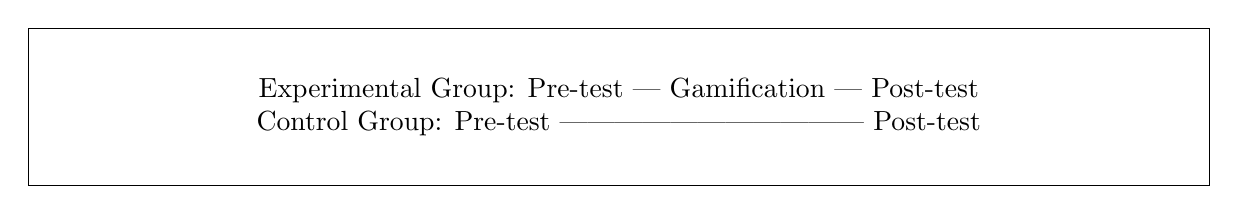
\begin{tikzpicture}
	\draw (-5, -1) rectangle (10,1);
	\node at (2.5,0) [align=center] {
		Experimental Group: Pre-test --- Gamification --- Post-test \\ 
		Control Group: Pre-test --------------------------------- Post-test
};
\end{tikzpicture}

\noindent Due to factors such as the difficulty of finding experimental subjects, the difficulty of developing gamification-related experimental facilities, and the time and cost of the experiment, this study does not consider Solomon's four-group experimental design.

\subsection*{- Population of Intereste}

\vspace{.3cm}

\noindent The experimental population of this study is all sociology undergraduate students in Trinity College Dublin's human science grouping. The reason for choosing this course is that this grouping has 640
\footnote[4]{
	This data is from Trinity College website:
	\url{https://www.tcd.ie/courses/search/?keywords=&type=undergraduate}.
}
vacannies, which means that we can have a large enough population to sample during the experiment. In addition, this courses have a varity range of classical social science subject like spychology, political science, sociology, ecnomics, etc. And Selecting students from one course rather than more also facilitates the unified setting and management of courses.

\subsection*{- Implementation of Experiment}

\vspace{.3cm}

\noindent Firstly, we need to confirm our sample size. Here are some default parameters:
\begin{equation}
	\alpha = 0.05, \beta = 0.2
\end{equation}
\begin{equation}
	1 - \beta = StatisticsPower = 0.8
\end{equation}
\noindent This study uses effect size from the previous literature. Trough literature review, Kim and Castelli have calculated an average effect size 
$\delta$ of gamification should be 0.25 \citep{kim2021effects}
\begin{equation}
	n = \frac{{2(Z_{\alpha/2} + Z_{\beta})^2 \sigma^2}}{{\delta^2}}
\end{equation}
Then we can calculate the require sample size should be 252 with 126 students in the experimental group and 126 students in the control group.
\par
\noindent This study will use simple random sampling method. The sampling frame is the list of all students provided by the social and human science school. In order to randomize, first we need to shuffle the order of all students on the list. This step is to prevent the list from being arranged according to certain rules, such as course, nationality, gender, etc. Then we will use a random number table to sample until the number of students in the experimental group and the control group is full. Once we have completed sampling, we will use the sample demographic characteristics to compare with the population to ensure that there is no significant difference in the proportion of gender, age, etc.\ between the sample and the overall population before making a final decision.

\subsection*{- Treatment and Manipulation}

\vspace{.3cm}

\noindent This experiment will offer an elective course on general concepts of social sciences in human science. The main reason for choosing elective courses is that experiments can be carried out without making drastic changes to the existing course structure, and it also facilitates subsequent ethical considerations. In addition, courses about general concepts are structured in such a way that the knowledge is relevant to students of all social sciences.

\noindent The experimental group and the control group will be taught the same content courses by the same teacher on two different days, but the experimental group will use game-based learning methods, while the control group will use traditional teaching methods. As mentioned in the \textit{theoretical argument} section, this article will use a set of gamification strategies, specifically including setting up an achievement system for students' learning progress, setting up customizable virtual images and assets for each student, a mutual aid system, and a graded system linked to learning.

\noindent Before the start of the course, both groups of students were given an exam as a pre-test to measure the students' knowledge reserve level before learning. At the end of the course, the same exam is used as a post-test to measure students' knowledge level after learning.

\subsection*{- Measure of Outcome Variable}

\vspace{.3cm}

\noindent There are two measures of outcome, one through end-of-semester exam scores and the other through interviews with students at the end of the semester. Among them, the difference between the final exam and the beginning exam scores of the experimental group and the control group will be calculated respectively, and a two-sample mean \texttt{t} test will be used to test whether gamification has significantly improved students' learning performance. At the same time, the researcher will also conduct interviews with the participating students, asking them whether their learning experience was good throughout the semester, and attached a scale for testing on intrinsic and extrinsic motivation for learning.

\noindent The final results will be measured using a combination of quantitative and qualitative materials, which respectively represent the objective and subjective improvement of gamification on students' learning efficiency. Ultimately, the objective learning efficiency evaluation \textemdash\ that is, the improved scores in the post-test compared to the pre-test \textemdash\ and the subjective learning efficiency evaluation \textemdash\ that is, the students' subjective feelings from the answers in the scale \textemdash\ will be added together to form a measure  of students' learning efficiency.

\subsection*{- Ethical Consideration}

\vspace{.3cm}

\noindent The experiment may have the following ethical issues regarding fairness: (1) students may feel unfair due to prior grouping; (2) students may not take elective courses seriously; (3) students may disatisficed because the elective courses are only for experimental design, not for the public.

\noindent To solve these problems, this study will: (1) At the beginning of the experiment, explain to students the purpose of the experiment, minor injustices that may occur during the experiment, information protection, post-event guarantee measures, etc., to dispel students' concerns. (2) Conduct relevant experimental meeting instructions to both students and teachers to ensure the professionalism and controllability of the process. (3) After the experiment ends, elective courses will be open to students who have not participated before to protect students' learning rights.

\subsection*{- Practicality and Feasibility}

\noindent The funding for this experiment is 5,000 \texteuro{} and the duration is one year.This research divided a year into three stages, each stage has its own central tasks.
\begin{enumerate}[topsep=0pt]
	\item \textbf{Prepare Stage} \textendash\ \textit{Michaelmas Term}
		\begin{enumerate}
			\item Find literature and update literature review and research theories sturcture.
			\item Clear detail research plan and group member meetings.
			\item Prepare qualitative interview outline.
			\item Conduct a pre-survey among political science undergraduate students, which has a similar background and experience compared with sociology student, and test the scale's validity.
		\end{enumerate}
	\item \textbf{Experiment Stage} \textendash\ \textit{Hilary Term}
		\begin{enumerate}
			\item Randomlised and sampling, 
			\item Decide the assistant candidate for the research, and start the formal experiment.
		\end{enumerate}
	\item \textbf{Analysis Stage} \textendash\ \textit{Trinity Term}
		\begin{enumerate}
			\item Check the results and inspect the data from experiment.
			\item Coding qualitative and quantitative data obtained from experiments.
			\item Start to write the final paper of experiment.
		\end{enumerate}
\end{enumerate}
\noindent Most of the research funding will be used for recruitment and training of personnel. In addition, some funds will also be used for gamification software development, teaching system formulation, etc. But overall, the funding of 5,000 \texteuro{} is completely sufficient.

\newpage

\section*{Conclusion}

\vspace{.5cm}

\noindent This research design was based on a review of past literature and the decision was made to conduct an experiment with gamification in the field of social sciences. Past literature shows the characteristics of attaching great importance to science and engineering subjects and despising humanities and social sciences. Therefore, the current field of gamification needs some applied experiments in social sciences. The results of this study are expected to fill the gap of gamification in the field of social sciences and provide new ideas for teaching methods and curriculum of social sciences.

\noindent However, this design also has some potential limitations. First, using the same method as gamification experimental design in the scientific field may cause some problems, such as different subject systems, course classifications, etc.; secondly, the population and sample design based on the Trinity College Dublin Social Sciences Group may lead to poor external validity. Low, it is difficult to generalize the conclusion.

\noindent In order to solve these problems, first of all, during the pre-research period, we should always pay attention to whether there are disciplinary differences in the adaptability of the survey; secondly, when summarizing the conclusions, we should pay more careful attention to the scope of the inferences of the conclusions. Compare the two theories and consider whether to conduct a longer-term follow-up survey to improve external validity.

\newpage

\bibliographystyle{agsm}
\bibliography{mybibliography}
\end{document}
